\section{Results}
\label{sec:results}

\subsection{Motor Friction Estimation}
\label{sec:results:motor_friction_estimation}
  

\begin{table}[h]
    \centering
    \begin{tabular}{lrr}
        \hline
        Parameter & Hip Motor & Knee Motor \\
        \hline
        Viscous friction coefficient (without Coulomb) [Nm⋅s/rad] & 0.003552 & 0.011612 \\
        Viscous friction coefficient (with Coulomb) [Nm⋅s/rad] & 0.001703 & 0.006124 \\
        Coulomb friction [Nm] & 0.010963 & 0.024127 \\
        MSE without Coulomb & 0.003203 & 0.005989 \\
        MSE with Coulomb & 0.000953 & 0.001967 \\
        \hline
    \end{tabular}
    \caption{Friction model parameters and mean squared errors (MSE) for both motors, comparing models with and without Coulomb friction.}
    \label{tab:results:motor_friction_parameters}
\end{table}

Mean squared errors (MSE) are calculated between the simulated theta values with estimated friction parameters and the measured theta values, as shown in figure \ref{fig:results:motor_friction_estimation:linear_regression_knee_motor} and \ref{fig:results:motor_friction_estimation:linear_regression_hip_motor}.



\begin{figure}[h]
    \centering
    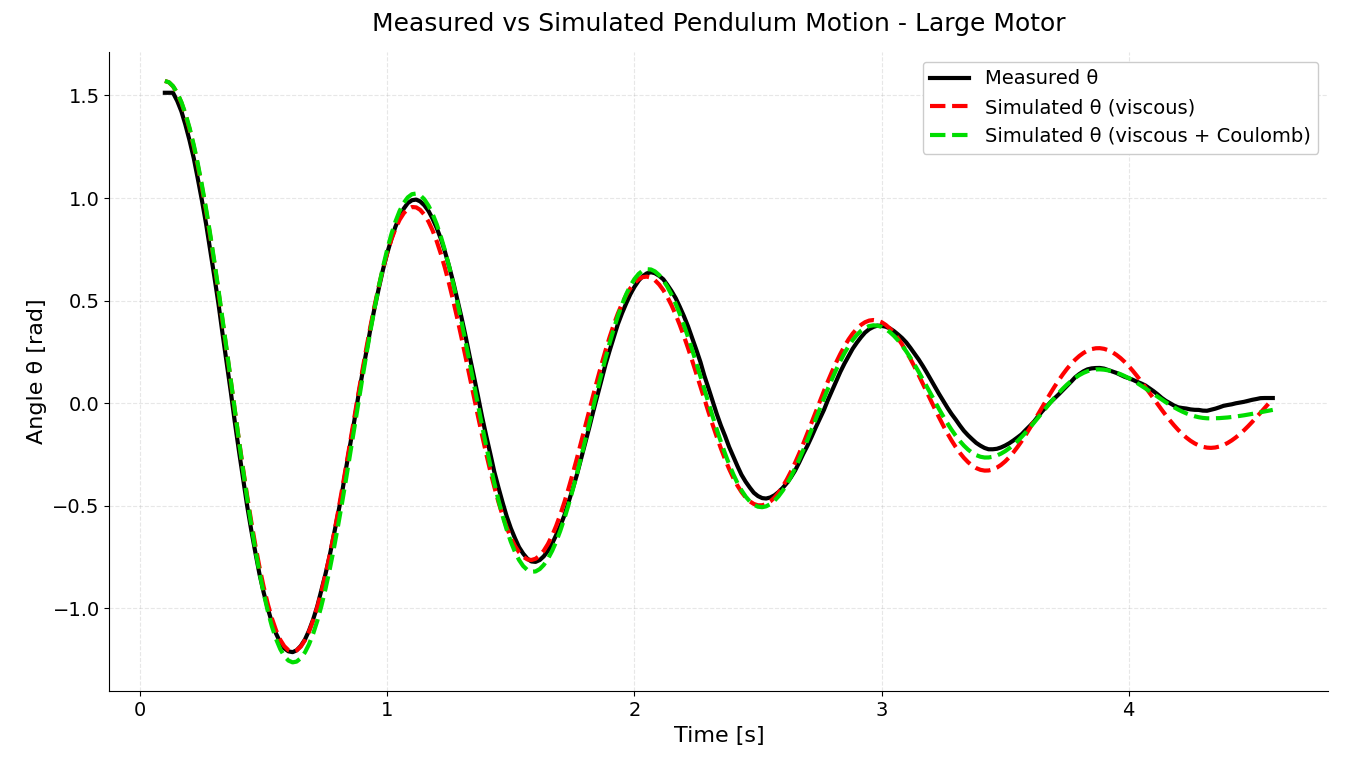
\includegraphics[width=0.8\textwidth]{Images/results/pendulum_large.png}
    \caption{Linear regression fit of the pendulum data for the knee motor. Derived theta dot dot is the double derivative of the pendulum angle.}
    \label{fig:results:motor_friction_estimation:pendulum_large}
\end{figure}

\begin{figure}[h]
    \centering
    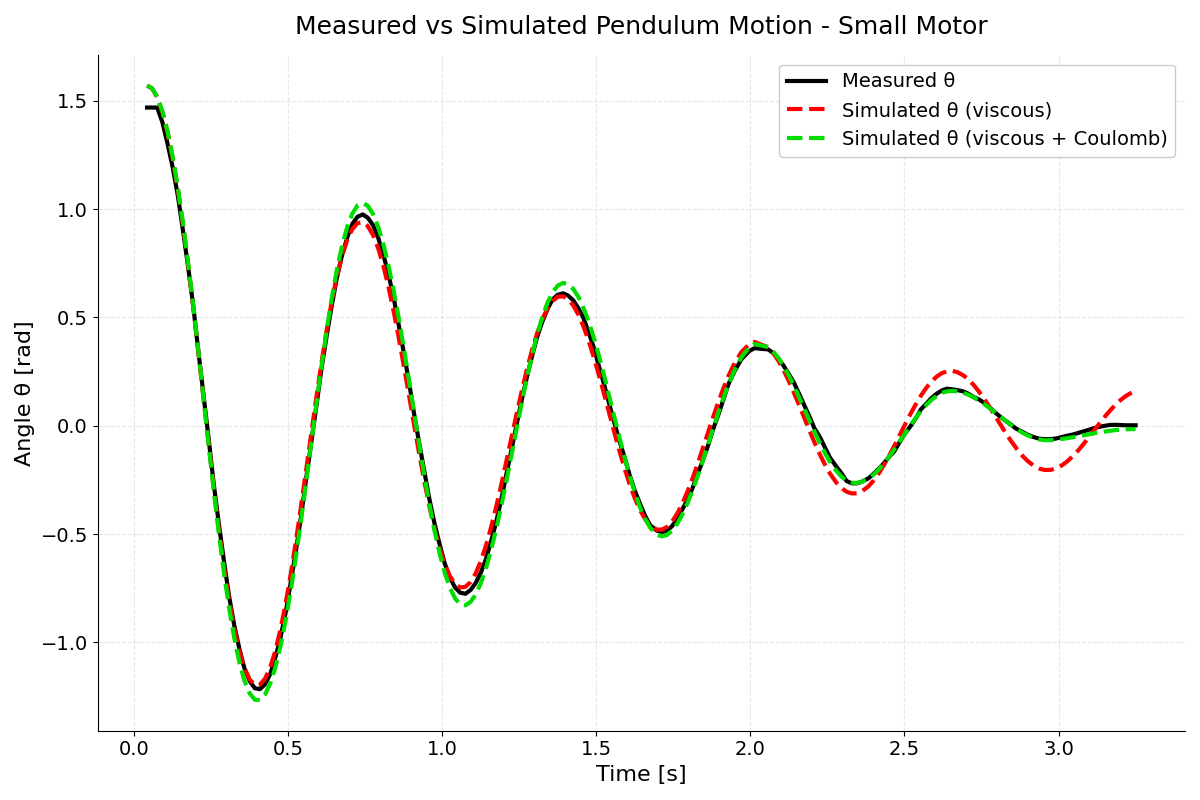
\includegraphics[width=0.8\textwidth]{Images/results/pendulum_small.png}
    \caption{Linear regression fit of the pendulum data for the hip motor.}
    \label{fig:results:motor_friction_estimation:pendulum_small}
\end{figure}




\subsection{Link Length Optimization}
\label{sec:results:link_length_optimization}
The grid search results for both Earth and Mars gravity are shown in figures \ref{fig:results:grid_search_earth} and \ref{fig:results:grid_search_mars}. The search explored link length ratios from 0.8 to 1.6 and total lengths from 8cm to 36cm, in increments of 0.1 and 0.5 cm respectively.

Best performing jumps are described in table \ref{tab:results:grid_search:best_jumps}.
\begin{table}[h]
    \centering
    \begin{tabular}{lrrrrr}
        \hline
        Gravity & Jump Height (cm) & Ratio & Total Length (cm) & L1 (cm) & L2 (cm) \\
        \hline
        Earth & 45.39 & 1.0 & 20 & 10 & 10 \\
        Mars & 149.79 & 1.0 & 28 & 14 & 14 \\
        \hline
    \end{tabular}
    \caption{Best performing link length configurations and their corresponding jump heights for Earth and Mars gravity.}
    \label{tab:results:grid_search:best_jumps}
\end{table}


\begin{figure}[h]
    \centering
    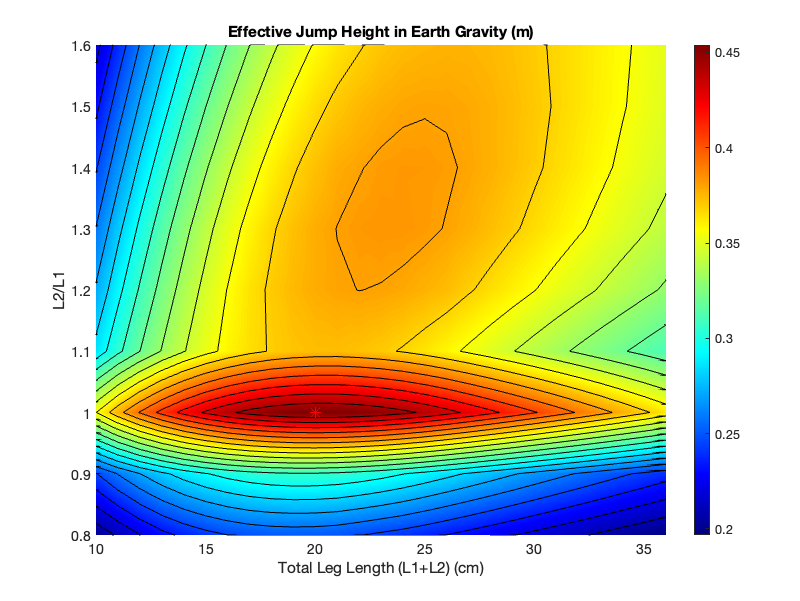
\includegraphics[width=0.8\textwidth]{Images/results/grid_search_earth.png}
    \caption{Grid search results showing jump height performance across different link length configurations under Earth gravity.}
    \label{fig:results:grid_search_earth}
\end{figure}



\begin{figure}[h]
    \centering
    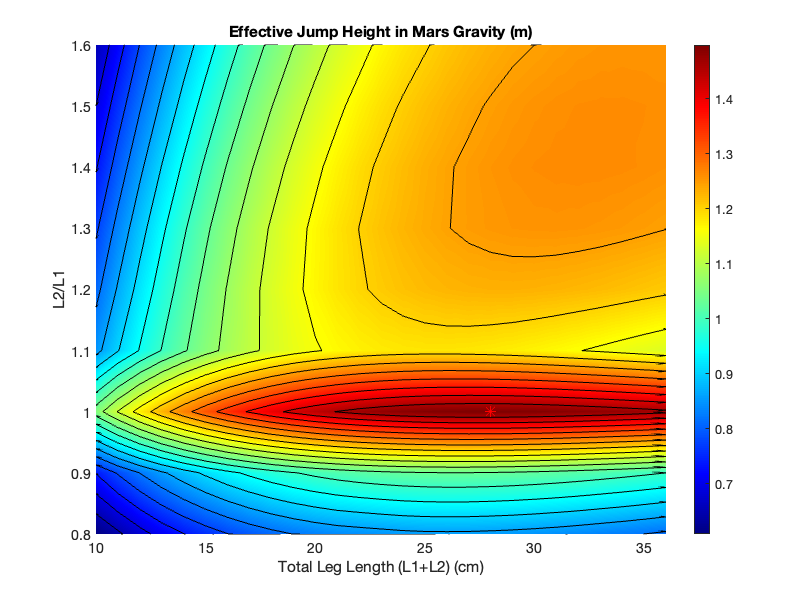
\includegraphics[width=0.8\textwidth]{Images/results/grid_search_mars.png}
    \caption{Grid search results showing jump height performance across different link length configurations under Mars gravity.}
    \label{fig:results:grid_search_mars}
\end{figure}

TODO: Correct optima
The optimum total length is 8cm longer under Mars gravity. In both Mars and Earth gravity, the optimal link length ratio is 1.0 across all total lengths, with steep drops in jump height for ratios under 1.0 and less steep drops for ratios over 1.0. 

\subsection{Hip Motor Dimensioning Test}
\label{sec:hip_motor_dimensioning_test}

As can be seen in figure \ref{fig:hip_motor_strength_test}, the hip motors follow the angle reference well, achieving three back and forth swings of 90 degrees over a one second period. The torque output of the motors during this maneuver can be seen in figure \ref{fig:hip_motor_torque_test}. In other words, the hip motors satisfy the heuristic as presented in \cite{finn_tarek_master}.

\begin{figure}[H]
    \centering
    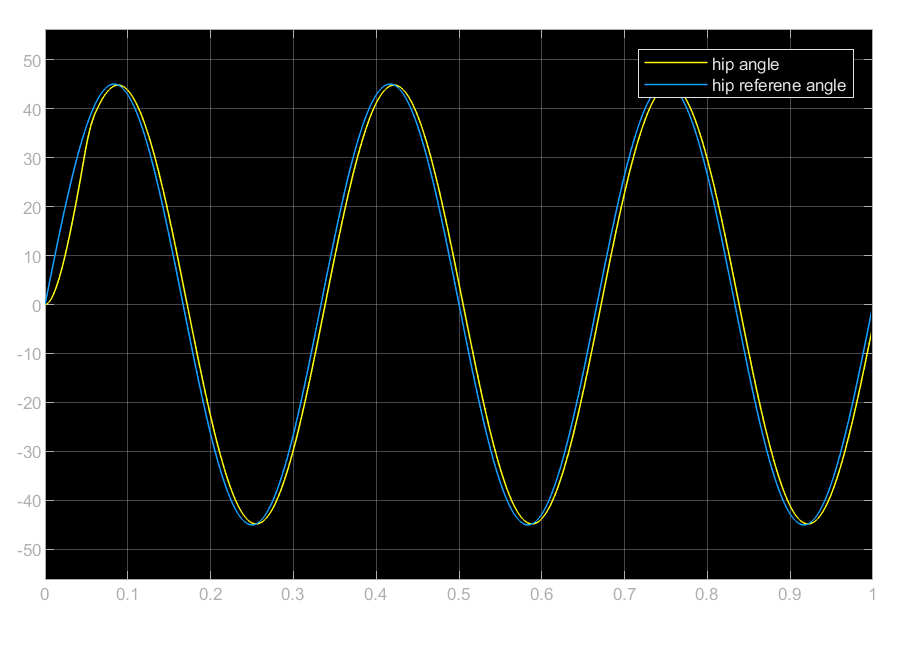
\includegraphics[width=0.8\textwidth]{Images/attitude_stable_test_result.eps}
    \caption{Commanded and actual hip joint angle achieved during the hip motor strength test simulation. }
    \label{fig:hip_motor_strength_test}
\end{figure}

\begin{figure}[H]
    \centering
    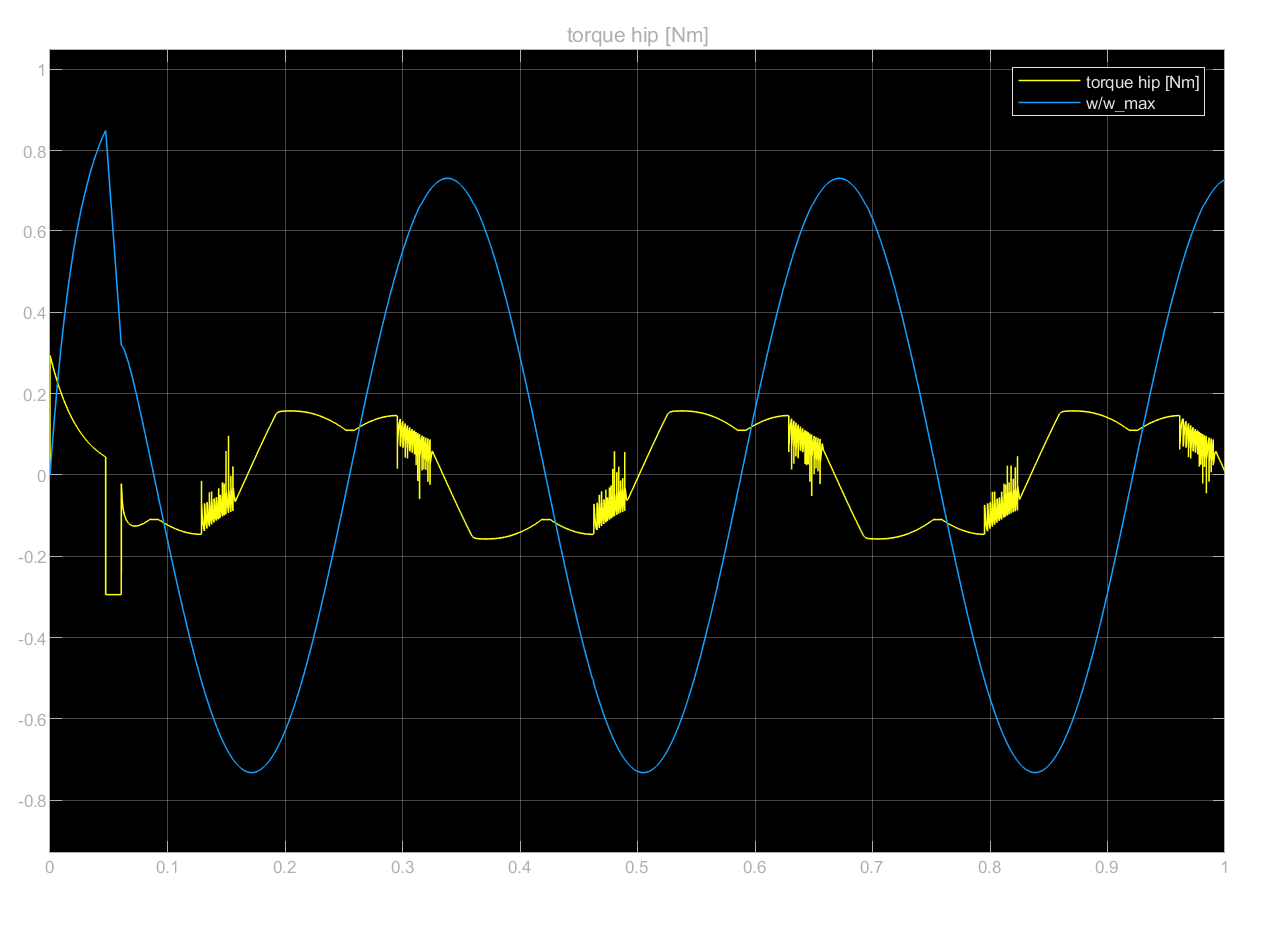
\includegraphics[width=0.8\textwidth]{Images/hip_motor_torque.eps}
    \caption{Torque output of the hip motors during the hip motor strength test simulation.}
    \label{fig:hip_motor_torque_test}
\end{figure}

\subsection{Motor Only Jumping Results}
\label{sec:results_motor_only_jumps}

As described in section \ref{sec:design_motor_only_jumps}, motor-only simulations were done using the assumed characteristics of the A80BHP-H motor. Because the results were so far from acceptable, only the results of one experiment are presented here, but simulations with shorter leg and body lengths were performed. Figure \ref{fig:joint_speed_A80BHM} shows the knee joint actuation torque, knee joint velocity and knee joint angle during takeoff for the A80BHP-H motor. The robot is not able to reach a high enough speed to achieve a good jump, and the peak body center of mass height reached is 70cm, despite a total leg length of 40cm.
% TODO: INclude below in results
%. These motors were chosen due to their high torque to weight ratio. While extensive testing was done, the jumping performance was so far from acceptable that the idea was abandoned, and the full scope of the experiments are considered outside the scope of this report. The best jumping performance was achieved with the A80BHP-H motor from AGF-RC. This motor has a stall torque of 18.5 kg/cm, a weight of 80 grams, and a maximum velocity of 2000 degrees per second. To test jumping performance, the robots dimensions were gradually increased, body length as well as link lengths. This gradual increase was terminated when the body length reached 30cm and the thigh and shank links reached 20cm each, for a total leg length of 40cm. The search was terminated here because the robot was still not jumping satisfactorily, despite the robots dimensions having reached a point where they were considered excessive. Primarily because the body mass was not being scaled with the general dimensions of the robot, and because the jump height was also not increasing at a commensurate rate with the increase in robot size. Ie., even though the total center of mass displacement was increasing, the center of mass jump height compared to the total length of the legs was not increasing, and the robot was thus not jumping higher. The achieved velocity of the knee joint until takeoff can be seen in figure \ref{fig:joint_speed_A80BHM}. As can be seen, the motor torque drops quickly, and is not able to reach a high enough speed to achieve a good jump. In fact, the peak body center of mass height reached is 70cm, despite a total leg length of 40cm. As can be seen, the motor is too slow to reach a high enough joint velocity for a good jump, it is therefore unlikely that a faster but weaker motor would perform much better. Efforts were made to test motors with both higher torques and higher speeds, but no motors were found with similar specs without being significantly heavier and larger. TODO: Should I show some motors that are objectively worse, as an example? 


\begin{figure}[h]
    \centering
    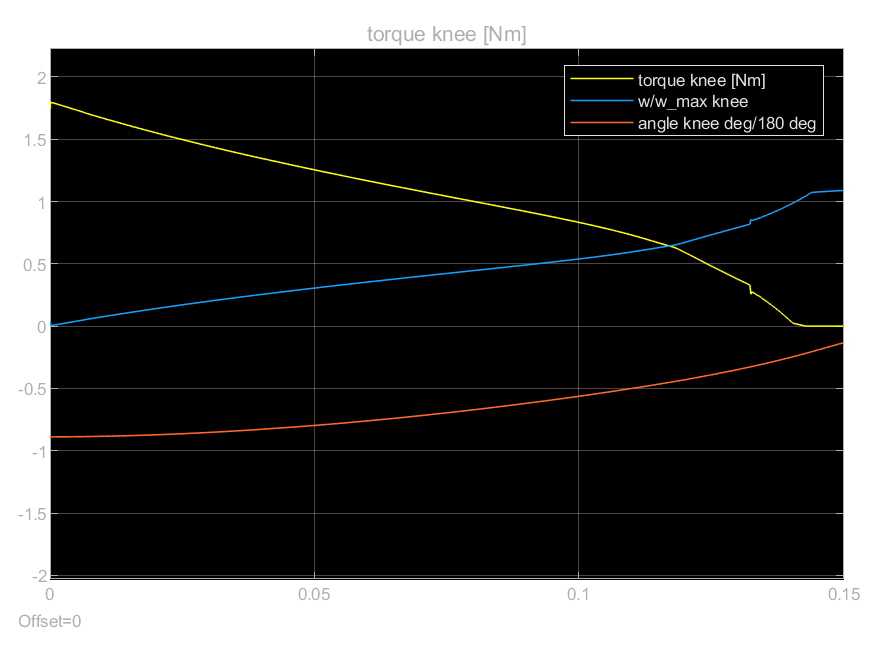
\includegraphics[width=0.75\textwidth]{Images/joint_speed_A80.eps}
    \caption{Knee speed until takeoff with A80BHP-H motor.}
    \label{fig:joint_speed_A80BHM}
\end{figure}
